\documentclass{beamer}
%\usepackage[ngerman]{babel}
\usepackage[T1]{fontenc}
\usepackage[utf8x]{inputenc}

%\setbeameroption{show notes on second screen=left}
%\setbeameroption{show notes on second screen}
%\usetheme{default}
%\useoutertheme{smoothbars} %overview at top
%\useinnertheme[shadow=true]{rounded} %grey preview of bullet points
%\beamersetuncovermixins{\opaqueness<1>{25}}{\opaqueness<2->{15}}

\usepackage{tikz}
\usetikzlibrary{arrows}
\tikzstyle{block} = [draw,fill=blue!20,minimum size=2em]
\tikzstyle{block2} = [draw,fill=red!20,minimum size=2em]
\tikzstyle{block3} = [draw,fill=white,minimum size=2em]

\usepackage{ifthen}

\title{Übungsblatt 1}
\subtitle{Algorithm Engineering}
\author{Waldemar Smirnow, Michael Stypa}
\institute{Universität Osnabrück}
\date{\today}

\begin{document}
\begin{frame}
    \titlepage
\end{frame}

%queue
%-first-in-first-out data structure
%-first-come-first-server processing of a queue
%-performs the function of a buffer
%-doesnt have a capacity
%-can be empty
%-queue underflow
%-queue overflow

%klassischen internen Implementierungen des Datentyps Stack besprochen
\section{Aufgabe 1.1a}
\begin{frame}
  \frametitle{Queue}
  \framesubtitle{}
  \begin{figure}
    \centering
    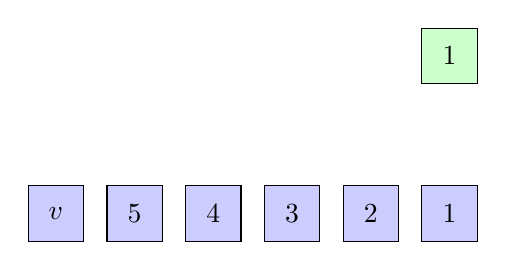
\begin{tikzpicture}
      \uncover<1-2>{\node[block] at (-1,0) (item1) {$1$};}
      \foreach \y [evaluate=\y as \x using \y-1] in {2,3,4,5} {
        \node[block] at (-\y,0) (item\y) {$\y$};
      }
      \uncover<2>{\node[block,fill=green!20] at (-6,0) (item6) {$v$};}
      \uncover<3->{\node[block] at (-6,0) (item6) {$v$};}
      \uncover<3->{\node[block,fill=green!20] at (-1,2) (item1) {$1$};}
    \end{tikzpicture}
  \end{figure}
  \begin{itemize}
    \item<2-> enqueue(type $v$) Hängt $v$ an den Anfang der Queue an
    \item<3-> type dequeue() Liefert ältestes Element der Queue und entfernt es
  \end{itemize}
\end{frame}

\begin{frame}
  \frametitle{Queue}
  \framesubtitle{Implementierungen (optimal im RAM-Modell)}
  Array + Zeiger auf oberstes Element + Zeiger auf unterstes Element
  \begin{figure}
    \centering
    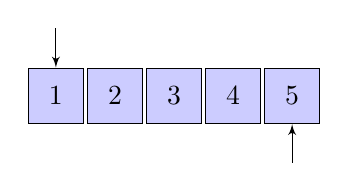
\begin{tikzpicture}[>=latex']
      \foreach \y in {1,2,3,4,5} {
        \node[block] at (3*\y/4,0) (item\y) {$\y$};
      }
      \draw[<-] (item1.north) -- +(0,0.5);
      \draw[<-] (item5.south) -- +(0,-0.5);
    \end{tikzpicture}
  \end{figure}

  Zeigerverkettete Liste
  \begin{figure}
    \centering
    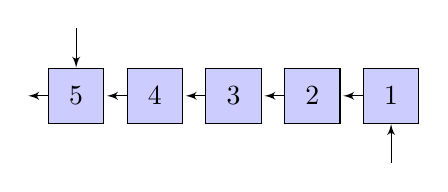
\begin{tikzpicture}[>=latex']
      \foreach \y in {1,2,3,4,5} {
        \node[block] at (-\y,0) (item\y) {$\y$};
        \draw[->] (item\y.west) -- +(-0.25,0);
      }
      \draw[<-] (item5.north) -- +(0,0.5);
      \draw[<-] (item1.south) -- +(0,-0.5);
    \end{tikzpicture}
  \end{figure}
\end{frame}

%ihr Verhalten im Externspeicher-Setting analysiert
\begin{frame}
  \frametitle{Queue}
  \framesubtitle{Verhalten im Externspeicher-Setting}
  $B=3$
  \begin{figure}
    \centering
    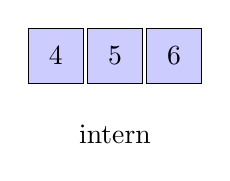
\begin{tikzpicture}[>=latex']
      \foreach \y in {4,5,6} {
        \node[block] at (3*\y/4,0) (item\y) {$\y$};
      }
      \node (d1) [below of=item5] {intern};
    \end{tikzpicture}
    \hspace{10mm}
    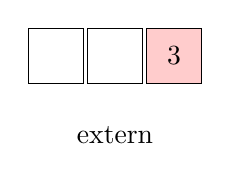
\begin{tikzpicture}[>=latex']
      \foreach \y in {1,2,3} {
        \ifthenelse{\y<3}
        {\node[block3] at (3*\y/4,0) (item\y) {};}
        {\node[block2] at (3*\y/4,0) (item\y) {$\y$};}
      }
      \node (d1) [below of=item2] {extern};
    \end{tikzpicture}
  \end{figure}
  Anzahl der I/Os (für beliebige Abfolge von Operationen)
  \begin{itemize}
    \item $O(1)$ pro Operation
  \end{itemize}
\end{frame}

%eine Modifikation vorgeschlagen, die in diesem Setting beweisbar besser funktioniert
\begin{frame}
  \frametitle{Extern-Queue}
  \framesubtitle{}
  \begin{itemize}[<+->]
    \item Interner Speicher ("Puffer"): Array $J$ der Größe $2B$; restliche Daten extern
    \item $J$ enthält zu jedem Zeitpunkt die zwei Blöcke mit Anfang und Ende der Queue
  \end{itemize}

  enqueue(type $v$)
  \begin{itemize}[<+->]
    \item Falls Anfang-Block Platz hat: Füge $v$ ein. Kein I/O
    \item Falls Anfang-Block voll: Vollen Anfang-Block auslagern und neuen im internen Speicher anfangen. 1 I/O
  \end{itemize}

  type dequeue($v$)
  \begin{itemize}[<+->]
    \item Falls Ende-Block mehr als einen Eintrag hat: $v$ ausliefern und aus dem Block löschen. Kein I/O
    \item Falls Ende-Block einen Eintrag hat: Eintrag ausliefern und neuen Ende-Block laden. 1 I/O
  \end{itemize}
\end{frame}

\end{document}
